\documentclass{article}
\usepackage{amsmath}
\usepackage{tikz}
\usetikzlibrary{calc,decorations.markings,decorations.pathmorphing,arrows.meta}
% set up externalization
\usetikzlibrary{external}
\tikzset{external/system call={latex \tikzexternalcheckshellescape -halt-on-error
-interaction=batchmode -jobname "\image" "\texsource";
dvips -o "\image".ps "\image".dvi;
ps2eps "\image.ps"}}
\tikzexternalize
\begin{document}
%---------------------------------------------------------------------------------
%
%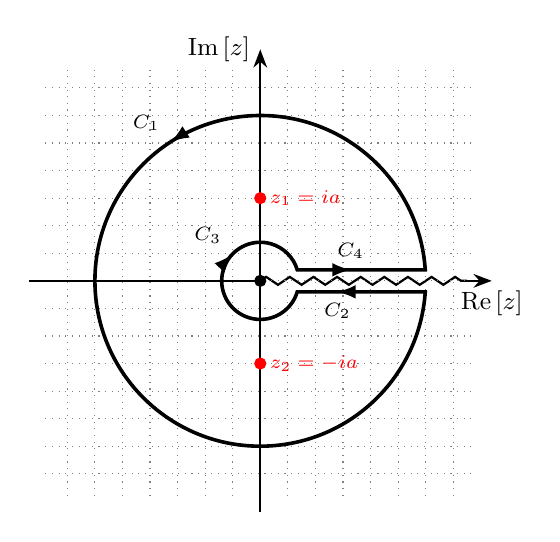
\begin{tikzpicture}[>=Latex,scale=0.7]
  % Configurable parameters
  \def\gap{0.4}
  \def\bigradius{3}
  \def\littleradius{0.7}
  \def\a{0.23}
  \def\b{0.74}
  \def\c{0.86}
  \def\d{0.95}
  %
  % Branch cut
  \draw[thick,
    decoration = {zigzag,segment length = 3mm, amplitude = 0.5mm},decorate]
    (0,0)--(1.25*\bigradius,0);
  %
  % Grid
  \draw[step=0.5cm,gray,dotted,thin] (-3.9,-3.9) grid (3.9,3.9);
  %
  % Axis
  \draw[thick] (-1.4*\bigradius, 0) -- (0,0);
  \draw[thick,-Stealth] (1.25 *\bigradius, 0) -- (1.4*\bigradius,0)
    node[below] {\small$\operatorname{Re}{[z]}$};
  \draw[thick,-Stealth] (0, -1.4*\bigradius) -- (0, 1.4*\bigradius)
    node[left] {\small$\operatorname{Im}{[z]}$};
  %
  % Contour path
  \draw[line width=1.3pt,   decoration={ markings,
    mark=at position \a with {\arrow[line width=.8pt]{>}},
    mark=at position \a with {\node[above left]{\scriptsize$C_1$};},
    mark=at position \b with {\arrow[line width=.8pt]{>}},
    mark=at position \b with {\node[below]{\scriptsize$C_2$};},
    mark=at position \c with {\arrow[line width=.8pt]{>}},
    mark=at position \c with {\node[above left]{\scriptsize$C_3$};},
    mark=at position \d with {\arrow[line width=.8pt]{>}},
    mark=at position \d with {\node[above]{\scriptsize$C_4$};}},
    postaction={decorate}]
    let
    \n1 = {asin(\gap/2/\bigradius)},
    \n2 = {asin(\gap/2/\littleradius)}
    in (\n1:\bigradius) arc (\n1:360-\n1:\bigradius)
    -- (-\n2:\littleradius) arc (-\n2:-360+\n2:\littleradius)
    -- cycle;
  %
  % Points
  \draw [fill] (0,0) circle [radius=0.1];
  \draw [fill,color=red] (0,1.5) circle [radius=0.1] node[right] {\scriptsize$z_1=ia$};
  \draw [fill,color=red] (0,-1.5) circle [radius=0.1] node[right] {\scriptsize$z_2=-ia$};
  %
\end{tikzpicture}
%
%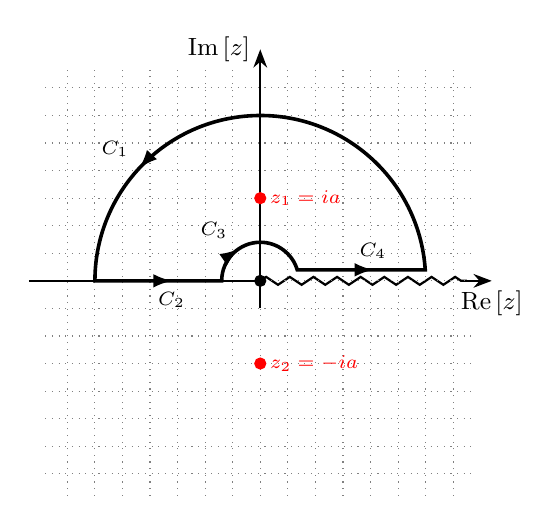
\begin{tikzpicture}[>=Latex,scale=0.7]
  % Configurable parameters
  \def\gap{0.4}
  \def\bigradius{3}
  \def\littleradius{0.7}
  \def\gap{0.4}
  \def\a{0.44}
  \def\b{0.67}
  \def\c{0.77}
  \def\d{0.94}
  %
  % Branch cut
  \draw[thick,
    decoration = {zigzag,segment length = 3mm, amplitude = 0.5mm},decorate]
    (0,0)--(1.25*\bigradius,0);
  %
  % Grid
  \draw[step=0.5cm,gray,dotted,thin] (-3.9,-3.9) grid (3.9,3.9);
  %
  % Axis
  \draw[thick] (-1.4*\bigradius, 0) -- (0,0);
  \draw[thick,-Stealth] (1.25 *\bigradius, 0) -- (1.4*\bigradius,0)
    node[below] {\small$\operatorname{Re}{[z]}$};
  \draw[thick,-Stealth] (0, -.5) -- (0, 1.4*\bigradius)
    node[left] {\small$\operatorname{Im}{[z]}$};
  %
  % Contour path
  \draw[line width=1.3pt,   decoration={ markings,
    mark=at position \a with {\arrow[line width=.8pt]{>}},
    mark=at position \a with {\node[above left]{\scriptsize$C_1$};},
    mark=at position \b with {\arrow[line width=.8pt]{>}},
    mark=at position \b with {\node[below]{\scriptsize$C_2$};},
    mark=at position \c with {\arrow[line width=.8pt]{>}},
    mark=at position \c with {\node[above left]{\scriptsize$C_3$};},
    mark=at position \d with {\arrow[line width=.8pt]{>}},
    mark=at position \d with {\node[above]{\scriptsize$C_4$};}},
    postaction={decorate}]
    let
    \n1 = {asin(\gap/2/\bigradius)},
    \n2 = {asin(\gap/2/\littleradius)}
    in (\n1:\bigradius) arc (\n1:180:\bigradius)
    -- (180:\littleradius) arc (180:\n2:\littleradius)
    -- cycle;
  %
  % Points
  \draw [fill] (0,0) circle [radius=0.1];
  \draw [fill,color=red] (0,1.5) circle [radius=0.1] node[right] {\scriptsize$z_1=ia$};
  \draw [fill,color=red] (0,-1.5) circle [radius=0.1] node[right] {\scriptsize$z_2=-ia$};
  %
\end{tikzpicture}
%
%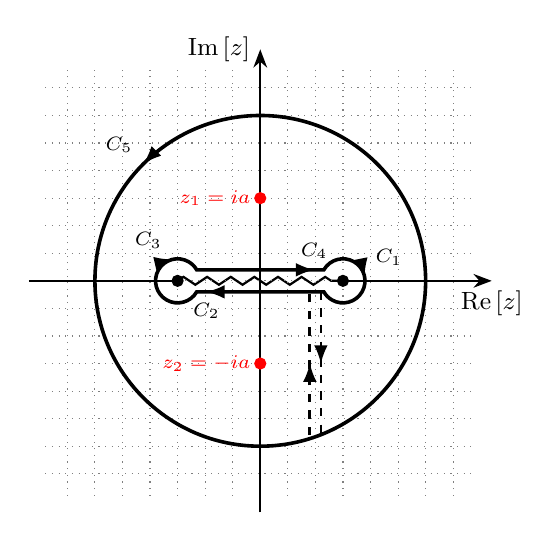
\begin{tikzpicture}[>=Latex,scale=0.7]
  % Configurable parameters
  \def\gap{0.4}
  \def\bigradius{3}
  \def\littleradius{0.4}
  \def\a{0.375}
  \def\b{0.11}
  \def\c{0.48}
  \def\d{0.68}
  \def\e{0.98}
  %
  % Branch cut
  \draw[thick,
    decoration = {zigzag,segment length = 3mm, amplitude = 0.5mm},decorate]
    (-1.5,0)--(1.5,0);
  %
  % Grid
  \draw[step=0.5cm,gray,dotted,thin] (-3.9,-3.9) grid (3.9,3.9);
  %
  % Axis
  \draw[thick] (-1.4*\bigradius,0) -- (-1.5,0);
  \draw[thick,-Stealth] (1.5,0) -- (1.4*\bigradius,0)
    node[below] {\small$\operatorname{Re}{[z]}$};
  \draw[thick,-Stealth] (0,-1.4*\bigradius) -- (0,1.4*\bigradius)
    node[left] {\small$\operatorname{Im}{[z]}$};
  %
  % Big circle contour
  \draw[line width=1.3pt,   decoration={ markings,
    mark=at position \a with {\arrow[line width=.8pt]{>}},
    mark=at position \a with {\node[above left]{\scriptsize$C_5$};}},
    postaction={decorate}] (0,0) circle [radius=\bigradius];
  %
  % Dog-bone contour
  \draw[line width=1.3pt,   decoration={ markings,
    mark=at position \b with {\arrow[line width=.8pt]{>}},
    mark=at position \b with {\node[above right]{\scriptsize$C_1$};},
    mark=at position \c with {\arrow[line width=.8pt]{>}},
    mark=at position \c with {\node[below]{\scriptsize$C_2$};},
    mark=at position \d with {\arrow[line width=.8pt]{>}},
    mark=at position \d with {\node[above left]{\scriptsize$C_3$};},
    mark=at position \e with {\arrow[line width=.8pt]{>}},
    mark=at position \e with {\node[above]{\scriptsize$C_4$};}},
    postaction={decorate}]
    let
    \n1 = {asin(\gap/2/\littleradius)}
    in ([shift=(180-\n1:\littleradius)]1.5,0) arc (180-\n1:-180+\n1:\littleradius)
    -- ([shift=(360-\n1:\littleradius)]-1.5,0) arc (360-\n1:+\n1:\littleradius)
    -- cycle;
  %
  % Connecting lines
  \draw[dashed, line width=1pt,   decoration={ markings,
    mark=at position 0.5 with {\arrow[line width=.8pt]{>}}},
    postaction={decorate}] (1.1,-\gap/2) -- (1.1,-\bigradius+0.2);
  \draw[dashed, line width=1pt,   decoration={ markings,
    mark=at position 0.5 with {\arrow[line width=.8pt]{>}}},
    postaction={decorate}] (0.9,-\bigradius+0.2) -- (0.9,-\gap/2);
  %
  % Points
  \draw [fill] (-1.5,0) circle [radius=0.1];
  \draw [fill] (1.5,0) circle [radius=0.1];
  \draw [fill,color=red] (0,1.5) circle [radius=0.1] node[left] {\scriptsize$z_1=ia$};
  \draw [fill,color=red] (0,-1.5) circle [radius=0.1] node[left] {\scriptsize$z_2=-ia$};
  %
\end{tikzpicture}
%
%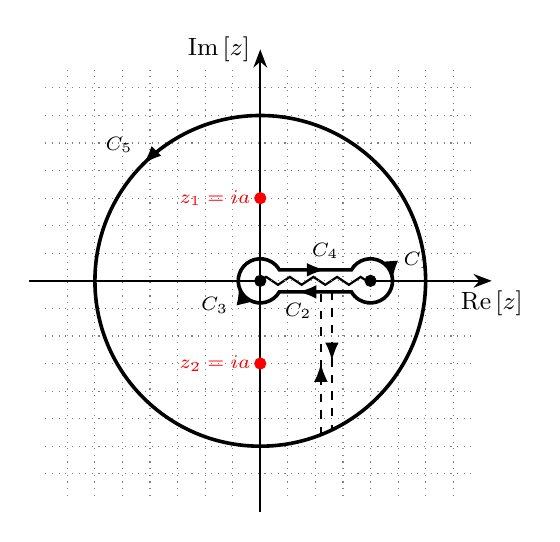
\begin{tikzpicture}[>=Latex,scale=0.7]
  % Configurable parameters
  \def\gap{0.4}
  \def\bigradius{3}
  \def\littleradius{0.4}
  \def\a{0.375}
  \def\b{0.15}
  \def\c{0.45}
  \def\d{0.64}
  \def\e{0.93}
  %
  % Branch cut
  \draw[thick,
    decoration = {zigzag,segment length = 3mm, amplitude = 0.5mm},decorate]
    (0,0)--(2,0);
  %
  % Grid
  \draw[step=0.5cm,gray,dotted,thin] (-3.9,-3.9) grid (3.9,3.9);
  %
  % Axes
  \draw[thick] (-1.4*\bigradius,0) -- (0,0);
  \draw[thick,-Stealth] (2,0) -- (1.4*\bigradius,0)
    node[below] {\small$\operatorname{Re}{[z]}$};
  \draw[thick,-Stealth] (0,-1.4*\bigradius) -- (0,1.4*\bigradius)
    node[left] {\small$\operatorname{Im}{[z]}$};
  %
  % Big circle contour
  \draw[line width=1.3pt,   decoration={ markings,
    mark=at position \a with {\arrow[line width=.8pt]{>}},
    mark=at position \a with {\node[above left]{\scriptsize$C_5$};}},
    postaction={decorate}] (0,0) circle [radius=\bigradius];
  %
  % Dog-bone contour
  \draw[line width=1.3pt,   decoration={ markings,
    mark=at position \b with {\arrow[line width=.8pt]{>}},
    mark=at position \b with {\node[above right]{\scriptsize$C_1$};},
    mark=at position \c with {\arrow[line width=.8pt]{>}},
    mark=at position \c with {\node[below]{\scriptsize$C_2$};},
    mark=at position \d with {\arrow[line width=.8pt]{>}},
    mark=at position \d with {\node[below left]{\scriptsize$C_3$};},
    mark=at position \e with {\arrow[line width=.8pt]{>}},
    mark=at position \e with { \node[above]{\scriptsize$C_4$};}},
    postaction={decorate}]
    let
    \n1 = {asin(\gap/2/\littleradius)}
    in ([shift=(180-\n1:\littleradius)]2,0) arc (180-\n1:-180+\n1:\littleradius)
    -- ([shift=(360-\n1:\littleradius)]0,0) arc (360-\n1:+\n1:\littleradius)
    -- cycle;
  %
  % Connecting lines
  \draw[dashed, line width=1pt,   decoration={ markings,
    mark=at position 0.5 with {\arrow[line width=.8pt]{>}}},
    postaction={decorate}] (1.3,-\gap/2) -- (1.3,-\bigradius+0.3);
  \draw[dashed, line width=1pt,   decoration={ markings,
    mark=at position 0.5 with {\arrow[line width=.8pt]{>}}},
    postaction={decorate}] (1.1,-\bigradius+0.2) -- (1.1,-\gap/2);
  %
  % Points
  \draw [fill] (0,0) circle [radius=0.1];
  \draw [fill] (2,0) circle [radius=0.1];
  \draw [fill,color=red] (0,1.5) circle [radius=0.1] node[left] {\scriptsize$z_1=ia$};
  \draw [fill,color=red] (0,-1.5) circle [radius=0.1] node[left] {\scriptsize$z_2=ia$};
  %
\end{tikzpicture}
%
%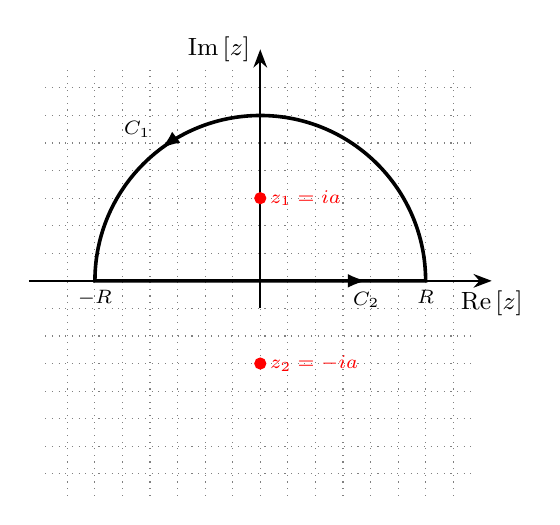
\begin{tikzpicture}[>=Latex,scale=0.7]
  % Configurable parameters
  \def\bigradius{3}
  \def\gap{0.4}
  \def\a{0.43}
  \def\b{0.93}
  %
  % Grid
  \draw[step=0.5cm,gray,dotted,thin] (-3.9,-3.9) grid (3.9,3.9);
  %
  % Axes
  \draw[thick,-Stealth] (-1.4*\bigradius,0) -- (1.4*\bigradius,0)
    node[below] {\small$\operatorname{Re}{[z]}$};
  \draw[thick,-Stealth] (0,-.5) -- (0,1.4*\bigradius)
    node[left] {\small$\operatorname{Im}{[z]}$};
  %
  % Contour path
  \draw[line width=1.3pt, decoration={markings,
    mark=at position \a with {\arrow[line width=.8pt]{>}},
    mark=at position \a with {\node[above left]{\scriptsize$C_1$};},
    mark=at position \b with {\arrow[line width=.8pt]{>}},
    mark=at position \b with {\node[below]{\scriptsize$C_2$};}},
    postaction={decorate}]
    (0:\bigradius) arc (0:180:\bigradius) -- cycle;
  %
  % Labels
  \node[below] at (-\bigradius,0) {\scriptsize$-R$};
  \node[below] at (\bigradius,0) {\scriptsize$R$};
  \draw [fill,color=red] (0,1.5) circle [radius=0.1] node[right] {\scriptsize$z_1=ia$};
  \draw [fill,color=red] (0,-1.5) circle [radius=0.1] node[right] {\scriptsize$z_2=-ia$};
  %
\end{tikzpicture}
%
%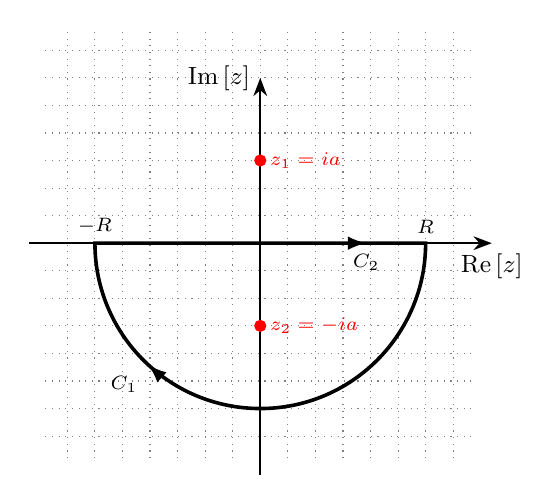
\begin{tikzpicture}[>=Latex,scale=0.7]
  % Configurable parameters
  \def\bigradius{3}
  \def\a{0.45}
  \def\b{0.93}
  %
  % Grid
  \draw[step=0.5cm,gray,dotted,thin] (-3.9,-3.9) grid (3.9,3.9);
  %
  % Axes
  \draw[thick,-Stealth] (-1.4*\bigradius, 0) -- (1.4*\bigradius,0)
    node[below] {\small$\operatorname{Re}{[z]}$};
  \draw[thick,-Stealth] (0,-1.4*\bigradius) -- (0,1*\bigradius)
    node[left] {\small$\operatorname{Im}{[z]}$};
  %
  % Contour path
  \draw[line width=1.3pt,   decoration={ markings,
    mark=at position \a with {\arrow[line width=.8pt]{>}},
    mark=at position \a with {\node[below left]{\scriptsize$C_1$};},
    mark=at position \b with {\arrow[line width=.8pt]{>}},
    mark=at position \b with {\node[below]{\scriptsize$C_2$};}},
    postaction={decorate}] (0:\bigradius) arc (0:-180:\bigradius)
    -- cycle;
  %
  % Labels
  \node[above] at (-\bigradius,0) {\scriptsize$-R$};
  \node[above] at (\bigradius,0) {\scriptsize$R$};
  \draw [fill,color=red] (0,1.5) circle [radius=0.1] node[right] {\scriptsize$z_1=ia$};
  \draw [fill,color=red] (0,-1.5) circle [radius=0.1] node[right] {\scriptsize$z_2=-ia$};
  %
\end{tikzpicture}
%
%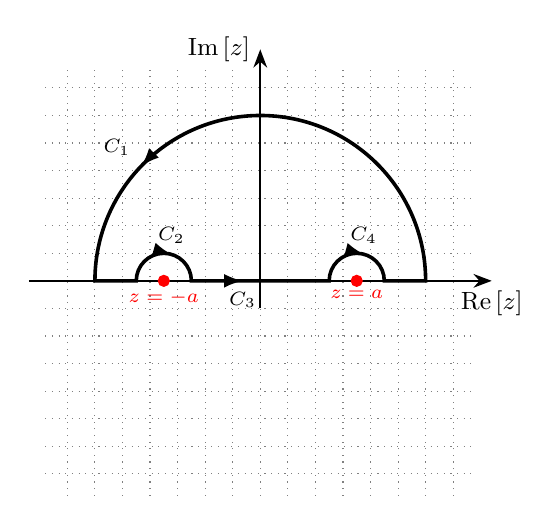
\begin{tikzpicture}[>=Latex,scale=0.7]
  % Configurable parameters
  \def\bigradius{3}
  \def\littleradius{0.5}
  \def\gap{0.4}
  \def\a{0.43}
  \def\b{0.67}
  \def\c{0.765}
  \def\d{0.915}
  %
  % Grid
  \draw[step=0.5cm,gray,dotted,thin] (-3.9,-3.9) grid (3.9,3.9);
  %
  % Axes
  \draw[thick,-Stealth] (-1.4*\bigradius,0) -- (1.4*\bigradius,0)
    node[below] {\small$\operatorname{Re}{[z]}$};
  \draw[thick,-Stealth] (0,-.5) -- (0,1.4*\bigradius)
    node[left] {\small$\operatorname{Im}{[z]}$};
  %
  % Contour path
  \draw[line width=1.3pt,   decoration={ markings,
    mark=at position \a with {\arrow[line width=.8pt]{>}},
    mark=at position \a with {\node[above left]{\scriptsize$C_1$};},
    mark=at position \b with {\arrow[line width=.8pt]{>}},
    mark=at position \b with {\node[above]{\scriptsize$C_2$};},
    mark=at position \c with {\arrow[line width=.8pt]{>}},
    mark=at position \c with {\node[below]{\scriptsize$C_3$};},
    mark=at position \d with {\arrow[line width=.8pt]{>}},
    mark=at position \d with {\node[above]{\scriptsize$C_4$};}},
    postaction={decorate}]
    (0:\bigradius) arc (0:180:\bigradius)
    -- ([shift=(180:\littleradius)]-1.75,0) arc (180:0:\littleradius)
    -- ([shift=(180:\littleradius)]1.75,0) arc (180:0:\littleradius)
    -- cycle;
  %
  % Points
  \draw [fill,color=red] (-1.75,0) circle [radius=0.1] node[below] {\scriptsize$z=-a$};
  \draw [fill,color=red] (1.75,0) circle [radius=0.1] node[below] {\scriptsize$z=a$};
  %
\end{tikzpicture}
%
%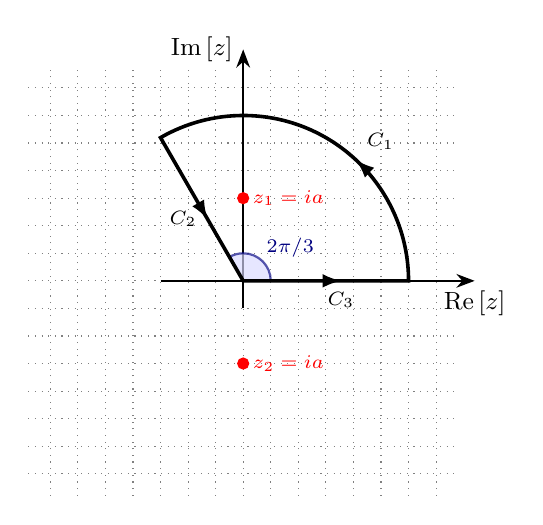
\begin{tikzpicture}[>=Latex,scale=0.7]
  % Configurable parameters
  \def\bigradius{3}
  \def\n1{120}
  \def\a{0.2}
  \def\b{0.65}
  \def\c{0.9}
  %
  % Grid
  \draw[step=0.5cm,gray,dotted,thin] (-3.9,-3.9) grid (3.9,3.9);
  %
  % Axes
  \draw[thick,-Stealth] (-1.5,0) -- (1.4*\bigradius,0)
    node[below] {\small$\operatorname{Re}{[z]}$};
  \draw[thick,-Stealth] (0,-0.5) -- (0, 1.4*\bigradius)
    node[left] {\small$\operatorname{Im}{[z]}$};
  %
  % Angle label
  \filldraw[fill=blue!15!white,opacity=0.65, draw=blue!50!black,thick]
    (0.5,0) arc (0:\n1:0.5) -- (0,0) -- cycle;
  \node[blue!50!black,above right] at (0.25,0.25) {\scriptsize$2\pi/3$};
  %
  % Contour path
  \draw[line width=1.3pt,   decoration={ markings,
    mark=at position \a with {\arrow[line width=.8pt]{>}},
    mark=at position \a with {\node[above right]{\scriptsize$C_1$};},
    mark=at position \b with {\arrow[line width=.8pt]{>}},
    mark=at position \b with {\node[left]{\scriptsize$C_2$};},
    mark=at position \c with {\arrow[line width=.8pt]{>}},
    mark=at position \c with {\node[below]{\scriptsize$C_3$};}},
    postaction={decorate}] (0:\bigradius) arc (0:\n1:\bigradius)
    -- (0,0) -- cycle;
  %
  % Points
  \draw [fill,color=red] (0,1.5) circle [radius=0.1] node[right] {\scriptsize$z_1=ia$};
  \draw [fill,color=red] (0,-1.5) circle [radius=0.1] node[right] {\scriptsize$z_2=ia$};
  %
\end{tikzpicture}
%
%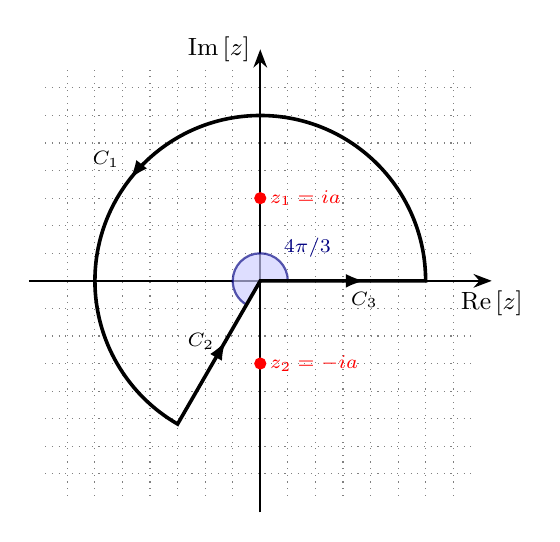
\begin{tikzpicture}[>=Latex,scale=0.7]
  % Configurable parameters
  \def\bigradius{3}
  \def\n1{240}
  \def\a{0.4}
  \def\b{0.77}
  \def\c{0.94}
  %
  % Grid
  \draw[step=0.5cm,gray,dotted,thin] (-3.9,-3.9) grid (3.9,3.9);
  %
  % Axes
  \draw[thick,-Stealth] (-1.4*\bigradius,0) -- (1.4*\bigradius,0)
    node[below] {\small$\operatorname{Re}{[z]}$};
  \draw[thick,-Stealth] (0,-1.4*\bigradius) -- (0, 1.4*\bigradius)
    node[left] {\small$\operatorname{Im}{[z]}$};
  %
  % Angle label
  \filldraw[fill=blue!20!white,opacity=0.65,draw=blue!50!black,thick]
    (0.5,0) arc (0:\n1:0.5) -- (0,0) -- cycle;
  \node[blue!50!black,above right] at (0.25,0.25) {\scriptsize$4\pi/3$};
  %
  % Contour path
  \draw[line width=1.3pt,   decoration={ markings,
    mark=at position \a with {\arrow[line width=.8pt]{>}},
    mark=at position \a with {\node[above left]{\scriptsize$C_1$};},
    mark=at position \b with {\arrow[line width=.8pt]{>}},
    mark=at position \b with {\node[left]{\scriptsize$C_2$};},
    mark=at position \c with {\arrow[line width=.8pt]{>}},
    mark=at position \c with {\node[below]{\scriptsize$C_3$};}},
    postaction={decorate}] (0:\bigradius) arc (0:\n1:\bigradius)
    -- (0,0) -- cycle;
  %
  % Points
  \draw [fill,color=red] (0,1.5) circle [radius=0.1] node[right] {\scriptsize$z_1=ia$};
  \draw [fill,color=red] (0,-1.5) circle [radius=0.1] node[right] {\scriptsize$z_2=-ia$};
  %
\end{tikzpicture}
%
%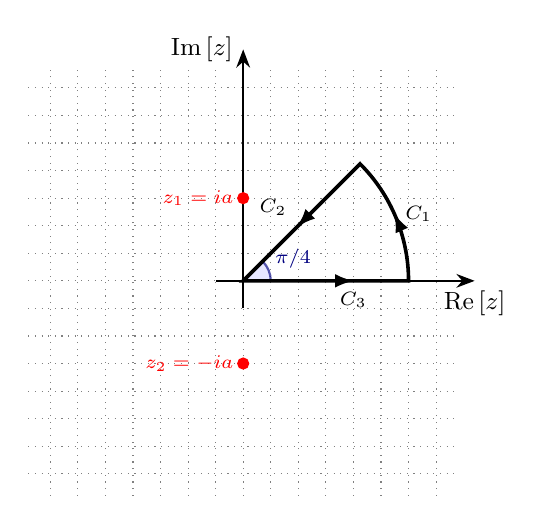
\begin{tikzpicture}[>=Latex,scale=0.7]
  % Configurable parameters
  \def\bigradius{3}
  \def\n1{45}
  \def\a{0.15}
  \def\b{0.475}
  \def\c{0.88}
  %
  % Grid
  \draw[step=0.5cm,gray,dotted,thin] (-3.9,-3.9) grid (3.9,3.9);
  %
  % Axes
  \draw[thick,-Stealth] (-0.5,0) -- (1.4*\bigradius,0)
    node[below] {\small$\operatorname{Re}{[z]}$};
  \draw[thick,-Stealth] (0,-0.5) -- (0, 1.4*\bigradius)
    node[left] {\small$\operatorname{Im}{[z]}$};
  %
  % Angle label
  \filldraw[fill=blue!15!white,opacity=0.65, draw=blue!50!black,thick]
    (0.5,0) arc (0:\n1:0.5) -- (0,0) -- cycle;
  \node[blue!50!black,above right] at (0.4,0.05) {\scriptsize$\pi/4$};
  %
  % Contour path
  \draw[line width=1.3pt, decoration={markings,
    mark=at position \a with {\arrow[line width=.8pt]{>}},
    mark=at position \a with {\node[right]{\scriptsize$C_1$};},
    mark=at position \b with {\arrow[line width=.8pt]{>}},
    mark=at position \b with {\node[above left]{\scriptsize$C_2$};},
    mark=at position \c with {\arrow[line width=.8pt]{>}},
    mark=at position \c with {\node[below]{\scriptsize$C_3$};}},
    postaction={decorate}]
    (0:\bigradius) arc (0:\n1:\bigradius) -- (0,0) -- cycle;
  %
  % Points
  \draw [fill,color=red] (0,1.5) circle [radius=0.1] node[left] {\scriptsize$z_1=ia$};
  \draw [fill,color=red] (0,-1.5) circle [radius=0.1] node[left] {\scriptsize$z_2=-ia$};
  %
\end{tikzpicture}
%
%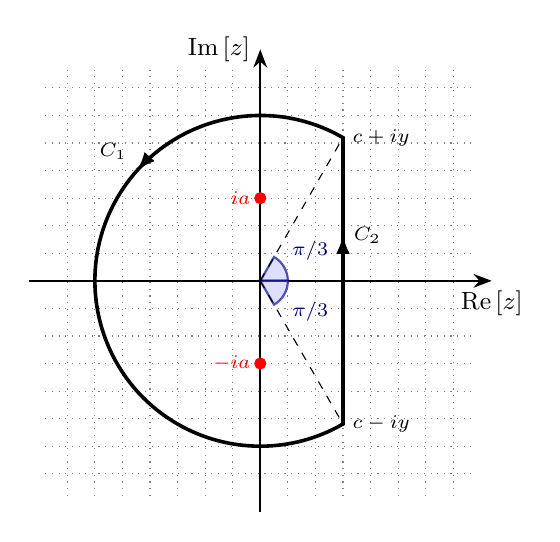
\begin{tikzpicture}[>=Latex,scale=0.7]
  % Configurable parameters
  \def\bigradius{3}
  \def\n1{60}
  \def\m2{300}
  \def\a{0.23}
  \def\b{0.9}
  %
  % Grid
  \draw[step=0.5cm,gray,dotted,thin] (-3.9,-3.9) grid (3.9,3.9);
  %
  % Axes
  \draw[thick,-Stealth] (-1.4*\bigradius,0) -- (1.4*\bigradius,0)
    node[below] {\small$\operatorname{Re}{[z]}$};
  \draw[thick,-Stealth] (0,-1.4*\bigradius) -- (0, 1.4*\bigradius)
    node[left] {\small$\operatorname{Im}{[z]}$};
  %
  % Angle label
  \filldraw[fill=blue!20!white,opacity=0.65,draw=blue!50!black,thick]
    (0.5,0) arc (0:\n1:0.5) -- (0,0) -- cycle;
  \node[blue!50!black,above right] at (0.4,0.2) {\scriptsize$\pi/3$};
  \filldraw[fill=blue!20!white,opacity=0.65,draw=blue!50!black,thick]
    (0.5,0) arc (0:\m2-360:0.5) -- (0,0) -- cycle;
  \node[blue!50!black,below right] at (0.4,-0.2) {\scriptsize$\pi/3$};
  %
  % Contour path
  \draw[line width=1.3pt,   decoration={ markings,
    mark=at position \a with {\arrow[line width=.8pt]{>}},
    mark=at position \a with {\node[above left]{\scriptsize$C_1$};},
    mark=at position \b with {\arrow[line width=.8pt]{>}},
    mark=at position \b with {\node[right]{\scriptsize$C_2$};}},
    postaction={decorate}]
    (\n1:\bigradius) arc (\n1:\m2:\bigradius) -- cycle;
  %
  % Connecting lines
  \draw[dashed] (0,0) -- (\n1:\bigradius);
  \draw[dashed] (0,0) -- (\m2:\bigradius);
  %
  % Labels
  \node[right] at (1.5,2.6) {\scriptsize$c+iy$};
  \node[right] at (1.5,-2.6) {\scriptsize$c-iy$};
  \draw [fill,color=red] (0,1.5) circle [radius=0.1] node[left] {\scriptsize$ia$};
  \draw [fill,color=red] (0,-1.5) circle [radius=0.1] node[left] {\scriptsize$-ia$};
  %
\end{tikzpicture}
%
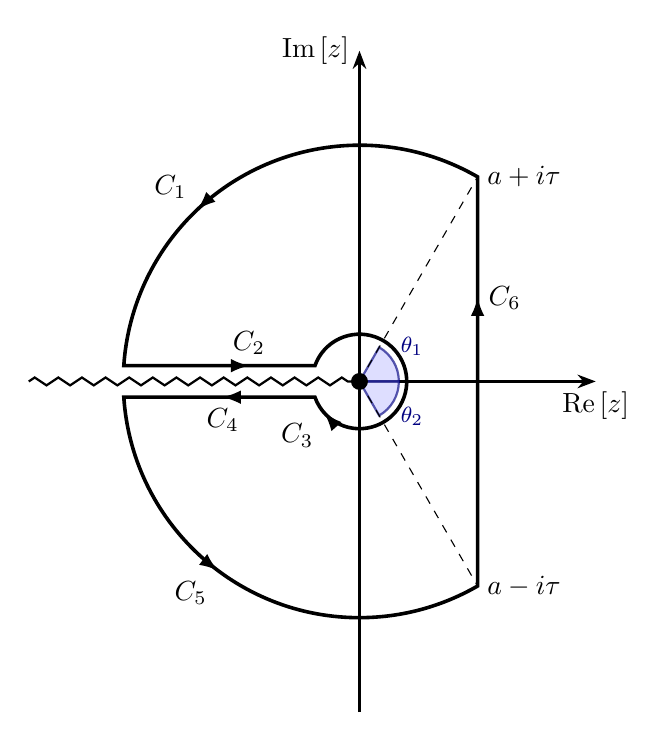
\begin{tikzpicture}[>=Latex,scale=1.0]
  % Configurable parameters
  \def\gap{0.4}             % Gap between contours above and below branch cut
  \def\bigradius{3}         % Radius of outer circular contour
  \def\littleradius{0.6}    % Radius of inner circular contour
  \def\upper{60}            % Angle at which vertical line intersects outer contour
  \def\a{0.15}              % C1
  \def\b{0.30}              % C2
  \def\c{0.455}              % C3
  \def\d{0.51}              % C4
  \def\e{0.66}              % C5
  \def\f{0.94}              % C6
  \newcommand{\axlables}{\normalsize}
  \newcommand{\annotations}{\normalsize}
  \newcommand{\anglables}{\footnotesize}
  %
  % Grid (uncomment below if necessary)
  %\draw[step=0.5cm,gray,dotted,thin] (-3.9,-3.9) grid (3.9,3.9);
  %
  % Branch cut
  \draw[thick,
    decoration = {zigzag,segment length = 3mm, amplitude = 0.5mm},decorate]
    (-1.4*\bigradius,0)--(0,0);
  % Axes
  \draw[thick,-Stealth] (0,0) -- (3,0)
    node[below] {\axlables$\operatorname{Re}{[z]}$};
  \draw[thick,-Stealth] (0,-1.4*\bigradius) -- (0, 1.4*\bigradius)
    node[left] {\axlables$\operatorname{Im}{[z]}$};
  %
  % Angle label
  \filldraw[fill=blue!20!white,opacity=0.65,draw=blue!50!black,thick]
    (0.5,0) arc (0:\upper:0.5) -- (0,0) -- cycle;
  \node[blue!50!black,above right] at (0.4,0.2) {\anglables$\theta_1$};
  \filldraw[fill=blue!20!white,opacity=0.65,draw=blue!50!black,thick]
    (0.5,0) arc (0:-\upper:0.5) -- (0,0) -- cycle;
  \node[blue!50!black,below right] at (0.4,-0.2) {\anglables$\theta_2$};
  % Contour path
  \draw[line width=1.3pt,   decoration={ markings,
    mark=at position \a with {\arrow[line width=.8pt]{>}},
    mark=at position \a with {\node[above left]{\annotations$C_1$};},
    mark=at position \b with {\arrow[line width=.8pt]{>}},
    mark=at position \b with {\node[above ]{\annotations$C_2$};},
    mark=at position \c with {\arrow[line width=.8pt]{>}},
    mark=at position \c with {\node[below left]{\annotations$C_3$};},
    mark=at position \d with {\arrow[line width=.8pt]{>}},
    mark=at position \d with {\node[below]{\annotations$C_4$};},
    mark=at position \e with {\arrow[line width=.8pt]{>}},
    mark=at position \e with {\node[below left]{\annotations$C_5$};},
    mark=at position \f with {\arrow[line width=.8pt]{>}},
    mark=at position \f with {\node[right]{\annotations$C_6$};}},
    postaction={decorate}]
    let
    \n1 = {asin(\gap/2/\bigradius)},
    \n2 = {asin(\gap/2/\littleradius)}
    in
    (\upper:\bigradius) arc (\upper:180-\n1:\bigradius)
    -- (180-\n2:\littleradius) arc (180-\n2:-180+\n2:\littleradius)
    -- (180+\n1:\bigradius) arc (180+\n1:360-\upper:\bigradius)
    -- cycle;
  %
  % Connecting lines
  \draw[dashed] (0,0) -- (\upper:\bigradius);
  \draw[dashed] (0,0) -- (-\upper:\bigradius);
  %
  % Labels
  \node[right] at (1.5,2.6) {\annotations$a+i\tau$};
  \node[right] at (1.5,-2.6) {\annotations$a-i\tau$};
  \draw [fill] (0,0) circle [radius=0.1];
  %
\end{tikzpicture}
%
%---------------------------------------------------------------------------------
\end{document}